\documentclass[a4paper,12pt]{exam}
%\printanswers % pour imprimer les réponses (corrigé)
\noprintanswers % Pour ne pas imprimer les réponses (énoncé)
\addpoints % Pour compter les points
% \noaddpoints % pour ne pas compter les points
%\qformat{\textbf{\thequestion ) } }
%\qformat{\textbf{\thequestion )}} % Pour définir le style des questions (facultatif)
\usepackage{color} % définit une nouvelle couleur
\shadedsolutions % définit le style des réponses
% \framedsolutions % définit le style des réponses
\definecolor{SolutionColor}{rgb}{0.8,0.9,1} % bleu ciel
\renewcommand{\solutiontitle}{\noindent\textbf{Solution:}\par\noindent} % Définit le titre des solutions
\usepackage{framed}
\definecolor{shadecolor}{gray}{0.95}
\definecolor{TFFrameColor}{rgb}{1,1,1}
\definecolor{TFTitleColor}{rgb}{0.5,0.5,0.5}




\usepackage{float}

\makeatletter

\def\maketitle{{\centering%
	\par{\huge\textbf{\@title}}%
	\par{\@date}%
	\par}}

\renewcommand{\thesection}{Exercice \arabic{section} }   

\renewcommand{\thesubsection}{Partie \Alph{subsection}.}   

\makeatother

%\lhead{NOM Pr\'enom :}
%\rhead{\textbf{Les r\'eponses doivent \^etre justifi\'ees et r\'edig\'ees}}
%\cfoot{\thepage / \pageref{LastPage}}

\floatstyle{ruled}
\newfloat{doc}{!ht}{lex}
\floatname{doc}{Doc.}


%\usepackage{../../pas-math}
%\usepackage{../../moncours}


%\usepackage{pas-cours}
%-------------------------------------------------------------------------------
%          -Packages nécessaires pour écrire en Français et en UTF8-
%-------------------------------------------------------------------------------
\usepackage[utf8]{inputenc}
\usepackage[frenchb]{babel}
%\usepackage{numprint}
\usepackage[T1]{fontenc}
%\usepackage{lmodern}
\usepackage{textcomp}
\usepackage[french, boxed]{algorithm2e}
\usepackage{hyperref}


%-------------------------------------------------------------------------------

%-------------------------------------------------------------------------------
%                          -Outils de mise en forme-
%-------------------------------------------------------------------------------
\usepackage{hyperref}
\hypersetup{pdfstartview=XYZ}
%\usepackage{enumerate}
\usepackage{graphicx}
\usepackage{multicol}
\usepackage{tabularx}
\usepackage{multirow}
\usepackage{color}
\usepackage{eurosym}


\usepackage{anysize} %%pour pouvoir mettre les marges qu'on veut
%\marginsize{2.5cm}{2.5cm}{2.5cm}{2.5cm}

\usepackage{indentfirst} %%pour que les premier paragraphes soient aussi indentés
\usepackage{verbatim}
\usepackage{enumitem}
\usepackage{booktabs}
\usepackage[usenames,dvipsnames,svgnames,table]{xcolor}

\usepackage{variations}

%-------------------------------------------------------------------------------


%-------------------------------------------------------------------------------
%                  -Nécessaires pour écrire des mathématiques-
%-------------------------------------------------------------------------------
\usepackage{amsfonts}
\usepackage{amssymb}
\usepackage{amsmath}
\usepackage{amsthm}
\usepackage{tikz}
\usepackage{xlop}
\usepackage[output-decimal-marker={,}]{siunitx}
%-------------------------------------------------------------------------------

%-------------------------------------------------------------------------------
%                  -Nécessaires pour écrire des formules chimiquess-
%-------------------------------------------------------------------------------

\usepackage[version=4]{mhchem}

%-------------------------------------------------------------------------------
% Pour pouvoir exploiter les fichiers directement dans beamer
\newcommand{\pause}{\ }
%-------------------------------------------------------------------------------
%                    - Mise en forme avancée
%-------------------------------------------------------------------------------

\usepackage{ifthen}
\usepackage{ifmtarg}


\newcommand{\ifTrue}[2]{\ifthenelse{\equal{#1}{true}}{#2}{$\qquad \qquad$}}

%\newcommand{\kword}[1]{\textcolor{red}{\underline{#1}}}
%-------------------------------------------------------------------------------

%-------------------------------------------------------------------------------
%                     -Mise en forme d'exercices-
%-------------------------------------------------------------------------------
%\newtheoremstyle{exostyle}
%{\topsep}% espace avant
%{\topsep}% espace apres
%{}% Police utilisee par le style de thm
%{}% Indentation (vide = aucune, \parindent = indentation paragraphe)
%{\bfseries}% Police du titre de thm
%{.}% Signe de ponctuation apres le titre du thm
%{ }% Espace apres le titre du thm (\newline = linebreak)
%{\thmname{#1}\thmnumber{ #2}\thmnote{. \normalfont{\textit{#3}}}}% composants du titre du thm : \thmname = nom du thm, \thmnumber = numéro du thm, \thmnote = sous-titre du thm

%\theoremstyle{exostyle}
%\newtheorem{exercice}{Exercice}
%
%\newenvironment{questions}{
%\begin{enumerate}[\hspace{12pt}\bfseries\itshape a.]}{\end{enumerate}
%} %mettre un 1 à la place du a si on veut des numéros au lieu de lettres pour les questions 
%-------------------------------------------------------------------------------

%-------------------------------------------------------------------------------
%                    - Mise en forme de tableaux -
%-------------------------------------------------------------------------------

\renewcommand{\arraystretch}{1.7}

\setlength{\tabcolsep}{1.2cm}

%-------------------------------------------------------------------------------



%-------------------------------------------------------------------------------
%                    - Racourcis d'écriture -
%-------------------------------------------------------------------------------
%Droites
\newcommand{\dte}[1]{$(#1)$}
\newcommand{\fig}[1]{figure $#1$}
\newcommand{\sym}{symétrique}
\newcommand{\syms}{symétriques}
\newcommand{\asym}{axe de symétrie}
\newcommand{\asyms}{axes de symétrie}
\newcommand{\seg}[1]{$[#1]$}
\newcommand{\monAngle}[1]{$\widehat{#1}$}
\newcommand{\bissec}{bissectrice}
\newcommand{\mediat}{médiatrice}
\newcommand{\ddte}[1]{$[#1)$}


% Angles orientés (couples de vecteurs)
\newcommand{\aopp}[2]{(\vec{#1}, \vec{#2})} %Les deuc vecteurs sont positifs
\newcommand{\aopn}[2]{(\vec{#1}, -\vec{#2})} %Le second vecteur est négatif
\newcommand{\aonp}[2]{(-\vec{#1}, \vec{#2})} %Le premier vecteur est négatif
\newcommand{\aonn}[2]{(-\vec{#1}, -\vec{#2})} %Les deux vecteurs sont négatifs

%Ensembles mathématiques
\newcommand{\naturels}{\mathbb{N}} %Nombres naturels
\newcommand{\relatifs}{\mathbb{Z}} %Nombres relatifs
\newcommand{\rationnels}{\mathbb{Q}} %Nombres rationnels
\newcommand{\reels}{\mathbb{R}} %Nombres réels
\newcommand{\complexes}{\mathbb{C}} %Nombres complexes


%Intégration des parenthèses aux cosinus
\newcommand{\cosP}[1]{\cos\left(#1\right)}
\newcommand{\sinP}[1]{\sin\left(#1\right)}


%Probas stats
\newcommand{\stat}{statistique}
\newcommand{\stats}{statistiques}


\newcommand{\homo}{homothétie}
\newcommand{\homos}{homothéties}


\newcommand{\mycoord}[3]{(\textcolor{red}{\num{#1}} ; \textcolor{Green}{\num{#2}} ; \textcolor{blue}{\num{#3}})}
%-------------------------------------------------------------------------------

%-------------------------------------------------------------------------------
%                    - Mise en page -
%-------------------------------------------------------------------------------

\newcommand{\twoCol}[1]{\begin{multicols}{2}#1\end{multicols}}


\setenumerate[1]{font=\bfseries,label=\textit{\alph*})}
\setenumerate[2]{font=\bfseries,label=\arabic*)}


%-------------------------------------------------------------------------------
%                    - Elements cours -
%-------------------------------------------------------------------------------

%Correction d'exercice
\newcommand{\exoSec}[2]{\subsection*{Exercice #1 page #2}}
%-------------------------------------------------------------------------------
%                    - raccourcis d'écriture -
%-------------------------------------------------------------------------------

%Mise en évidence de termes clés
\newcommand{\mykw}[1]{\textcolor{red}{\underline{\textbf{#1}}}}

%Exercices
\newcommand{\exo}[2]{exercice #1 page #2}
\newcommand{\Exo}[2]{Exercice #1 page #2}

\renewcommand{\pause}{\ }

%Intervalles
\newcommand{\interOO}[2]{$]$#1 , #2$[$}
\newcommand{\interOF}[2]{$]$#1 , #2$]$}
\newcommand{\interFO}[2]{$[$#1 , #2$[$}
\newcommand{\interFF}[2]{$[$#1 , #2$]$}



%\usepackage{fullpage}
\author{\ }
\date{18 Janvier 2019}
\title{Brevet Blanc Sciences Physiques}


\begin{document}
%	\usepackage{fancyhdr}
%	
%	\pagestyle{fancy}
%	\fancyhf{}
	%\rhead{Share\LaTeX}

\begin{center}
	%\centering
	
	{\scshape\LARGE \textbf{DIPLÔME NATIONAL DU BREVET} \par}
	\vspace{1cm}
	{\scshape\Large \textbf{SESSION 2019}\par}
	\vspace{1.5cm}
	

	\begin{large}
		\begin{tabular}{|@{\ }c@{\ }|@{\ }c@{\ }|}
		\hline
		%\ & \ \\
		\'Epreuve : \textbf{PHYSIQUE-CHIMIE} & Série : \textbf{Générale} \\ \hline
		\ & \ \\
		Durée de l'épreuve : \textbf{30 mnutes} & 50 points \\ 
		\ & \ \\
		\hline
	\end{tabular}
	\end{large}
		
	\vspace{1cm}
	{\large\bfseries \'EPREUVE DU VENDREDI 18 JANVIER 2019}
	
	\vspace{1cm}
	{\itshape L'usage d'une calculatrice est autorisé\par}
	%\vfill
	\vspace{1.5cm}
	{\bfseries Ce sujet comporte \pageref{LastPage} pages numérotées de 1/\pageref{LastPage} à \pageref{LastPage}/\pageref{LastPage} }
	
%	\vspace{0.5cm}
%	{\bfseries Ce sujet comporte x annexes situés pages \pageref{annexe} /\pageref{LastPage} à \pageref{LastPage}/\pageref{LastPage} à remettre avec la copie.}
	
	\vspace{0.5cm}
	{\bfseries\itshape Le candidat doit s'assurer que le sujet distribué est complet. }
	
	%\vfill	
	
	%\fbox{
%		\begin{minipage}{0.9\textwidth}
%			\large
%			Il  est  rappelé  que  la  qualité  de  la  rédaction,  la  clarté  et  la  précision  des  raisonnements entreront pour une part importante dans l'appréciation des copies. 
%			
%			Cependant, le candidat est invité à faire figurer sur la copie toute trace de recherche, même incomplète ou infructueuse, qu'il aura développée. 
%		\end{minipage}
%	}
	
	%\vfill

% Bottom of the page
	%{\large \today\par}
\end{center}
\newpage
	
L'athlète sud africain Oscar PISTORIUS est le premier amputé des membres inférieurs à participer en 2012 aux jeux olympiques en compagnie d'athlètes non handicapés.\\

Pour cela Oscar PISTORIUS  utilise des prothèses CHEETAH (nom inspiré de l'animal le plus rapide de la planète : le guépard) développées par la société islandaise \"{O}ssur.
	
	
\vspace*{1cm}	

\begin{figure}
	\caption{Les performances d'Oscar PISTORIUS}
	\label{doc:perfs}
	
	
	\begin{shaded*}
		%\begin{minipage}{0.9\textwidth}
			Troisième aux jeux paralympiques de 2004, Oscar PISTORIUS remporte la finale du 200 mètres, avec un temps de 21 s 97. Ses prothèses, d'un coût supérieur à \num{20000} € lui font perdre du temps au départ. Il a aussi du mal à négocier les virages.
		%\end{minipage}
	\end{shaded*}
\end{figure} 	


\begin{doc}
	\label{doc:cheetah}
	\caption{Les Cheetah}
	
		\begin{quotation}
			Les \emph{Cheetah} sont constitués de fibres de carbone imprégnées de résine et collées les unes aux autres (30 à 90 selon la corpulence du porteur). Le tout est enfin pressé contre le moule d'une jambe afin d'en épouser la silhouette. La prothèse est ensuite chuaffée pour faire fondre la résine, celle-ci permettant d'évacuer les bulles d'air, causes de cassures.
	
	{\small Source : www.sciencesetavenir.fr}
		\end{quotation}
	
\end{doc}

\begin{doc}
	\label{doc:carbone}
	\caption{Les fibres de carbone}
	
\begin{quotation}
		Les fibres de carbone sont constituées essentiellement d'atomes de carbone C. 
	Avec un diamètre compris entre 5 et 7 micromètres et une masse volumique de l'ordre de $\num{1.8} \: g/cm^3$, ces fibres sont groupées sous forme de fils contenant de \num{1000} à \num{48000} ou plus.
	Ce matériau est caractérisé par sa faible densité (\num{1.7} à \num{1.9}), sa résistance élevée à la traction et à la compression, sa flexibilité, sa bonne conductivité électrique et thermique, sa tenue en température et son inertie chimique.
	Plus solide que l'acier, et plus léger que l'aluminium, ces fibres ne rouillent pas comme le fer et résistent à la chaleur. 
\end{quotation}
\end{doc}	


\begin{doc}
	\label{doc:oxydation}
	\caption{L'acier et l'aluminium}
	
	\begin{quotation}
	
	
	La rouille (hématite $Fe_2O_3$) de couleur brun-rouge est produite par la corrosion du fer ou des métaux contenant du fer comme l'acier.
	L'acier a une masse volumique $\rho_{acier}=\num{7.8} \: g/cm^3$ tandis que l'aluminium a une masse volumique de $\rho_{Al}=\num{2.7} \: g/cm^3$.
\end{quotation}
\end{doc}

%\vspace*{-0.5cm}	

\newpage
\begin{questions}
	\question Calculer la vitesse d'Oscar PISTORIUS lors des jeux paralympiques de 2004 en $m/s$ et en $km/h$.
	
	\question Dans le document 3, il est dit que les fibres de carbone sont plus légères que l'aluminium. Démontrer cette information à l'aide des documents 3 et 4.
	
	\question 
		\begin{parts}
			\part Donner le nom des deux constituants d'un noyau atomique.
			
			\part Le fer $_{26}Fe$ contient 56 nucléons. Donner le nombre des constituants du noyau ainsi que le nombre des électrons de l'atome de fer. Justifier.
			
			\part La rouille résulte de la réaction chimique entre le fer et et l'un des composants de l'air, lequel ?
		\end{parts} 
	
	
	\question On considère que les différentes parties de la prothèse Cheetah nécessitent environ 300 $cm^3$ de fibres de carbone.
		\begin{parts}
			\part Calculer la masse d'une prothèse en fibres de carbone.
			
			\part Calculer la masse de cette prothèse sil elle était en acier. Donner la réponse en $kg$, comparer les masses trouvées dans la question \textbf{4.} et conclure sur la raison de l'utilisation des fibres de carbone dans les prothèses Cheetah.
		\end{parts}	
			
\end{questions}

%\section{\'Equations de réaction}

Ajuster les équations de réactions suivantes :
\begin{questions}
	\question $CH_4 + ....O_2 \rightarrow ....CO_2 + ....H_2O$
	
	\question $C_7H_{16} + ....O_2 \rightarrow ....CO_2 + ....H_2O$	
	
	\question $C_6H_{2}O + ....O_2 \rightarrow ....CO_2 + ....H_2O$
\end{questions}

%
%\section{À chaque modèle sa formule}
\begin{questions}
	\question \'A partir de ces dessins de modèles, donner la formule des molécules suivantes.

	\begin{center}
		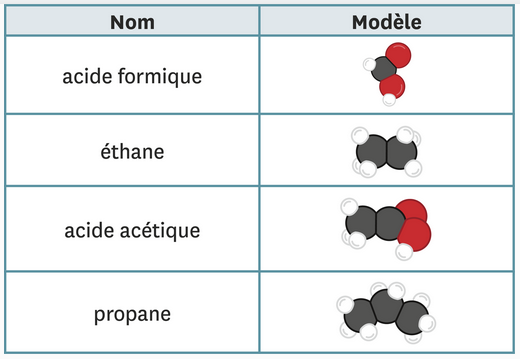
\includegraphics[scale=0.6]{img/exemples}
	\end{center}
	\fillwithdottedlines{2cm}
	
\end{questions}

%\section{Composition des molécules}


\begin{questions}
	\question Donner la composition des molécules suivantes :
	
	\begin{parts}
		\part l'éthylène $C_2H_4$	
		\fillwithdottedlines{1cm}
		
		\part le monoxyde d'azote $NO$	
		\fillwithdottedlines{1cm}
		
		\part l'ozone $O_3$	
		\fillwithdottedlines{1cm}	
		
		\part l'eau oxygénée $H_2O_2$	
		\fillwithdottedlines{1cm}
	\end{parts}

\end{questions}


%\newpage





 
%\newpage
%
%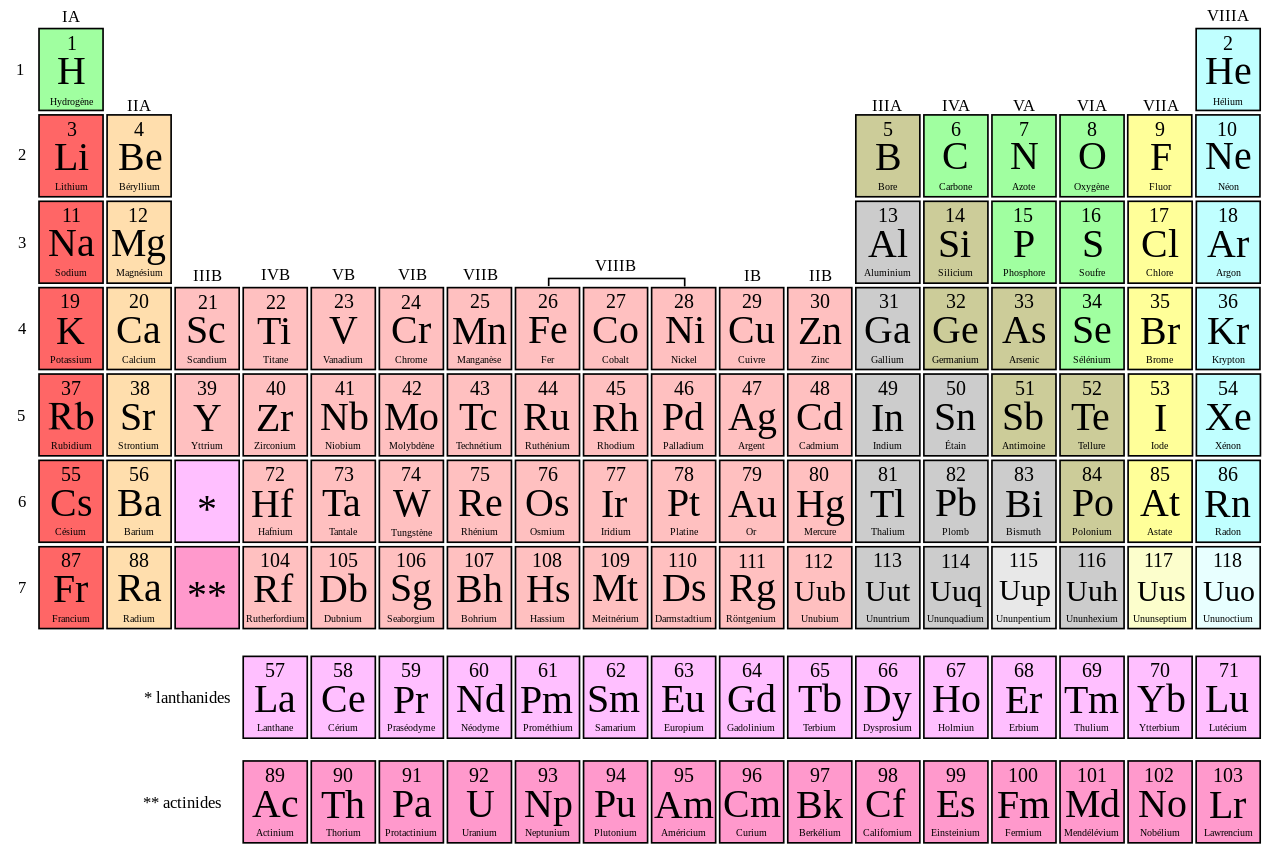
\includegraphics [scale=0.5, angle= 90 ]{img/tableau} 
\ \label{LastPage}

\end{document}